
\chapter{Introduccion}
\section{Breve prefacio del autor}
\begin{wrapfigure}{l}{0.25\textwidth}
	\centering
	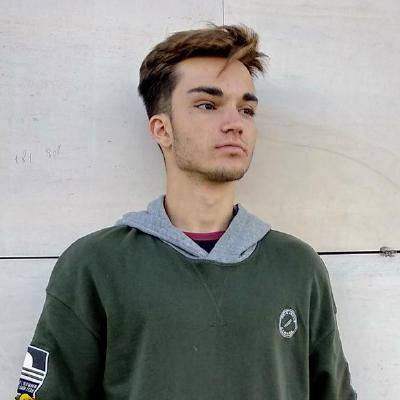
\includegraphics[width=0.25\textwidth]{figures/mi_foto.jpeg}
	\caption{una foto de cuando era joven...}
\end{wrapfigure}

Soy un estudiante de Ingenieria informatica en la universidad complutense de madrid. Nunca he encajado demasiado bien en los grupos de gente, suelo tener opiniones distintas al resto, esto sumado a algunas complicaciones en mi vida de adolescente, me ha llevado a pasar algunas temporadas de soledad, que he disfrutado pues he podido reflexionar a cerca de muchisimos temas que ardian dentro de mi, y darme cuenta de lo que para mi es realmente importante. 
Normalmente este tipo de periodos se daba en epocas vacacionales, pero debido al fuerte confinamiento que hemos vivido en Espana y a la politica personal que estoy llevando ante la situacion sanitaria, he tenido mucho tiempo para esta tarea. Ha sido un tiempo para llevar a cabo lecturas que tenia pendientes y atender clases y discursos de importantes mentores o personas con una opinion distinta a la gente en general.
Estos factores sumados a mi fuego interno y mi necesidad de no dejar las cosas para otro dia, por que si no nunca las hago, ha surgido la idea de escribir estas paginas, mientras caminaba por el campo tranquilamente.
Solo espero que la lectura sea recibida con la mente abierta, pues lo requiere. En mi experiencia, en estos momentos de soledad en los que considero que he crecido como persona, estableciendo quien soy , hacia donde voy y por que principios me rijo, lo he podido hacer por que estaba abierto al cambio. 
\section{Marco de \LaTeX}
Estas paginas se entregaran como un ejercicio final de el curso de latex (basix) que se imparte en la universidad Complutense de Madrid. Aunque el profesor nos pidio que fuera algo creativo, a mi me ha salido hacer esto, he intentado aplicar varias de las tecnicas que vimos dentro del curso para que se ajuste a los requisitos en cuanto al formato, pero en cuanto a contenido ha quedado un ejercicio mas serio, pero sentia la necesidad de hacerlo y asi ha sido. Aun asi creo que ha quedado un formato de <<libro>> improvisado distinto a lo normal con cosas un poco random por aqui y por alli que enriquecen el ejercicio con estas tecnicas de \LaTeX \\

Comentar que el ejercicio lo he elaborado en su mayoria \textit{offline} con un editor de texto y el paquete \textit{texlive-full} de linux. El codigo esta disponible en \href{https://github.com/dlgeraghty/basix-latex/tree/master/independencia/template}{mi github} \\

Para la documentacion basicamente he utilizado las guias que proporciona overleaf \textbf{INSERTAR REFERENCIA AQUI}
